\documentclass[../thesis.tex]{subfiles}

% graphics path
\graphicspath{
  {../../figures/chapter3/}
}

\begin{document}
\chapter{Developing Vapor Intrusion Models}

% TODO: Restructure to reflect the COMSOL workflow
% - Keep main body simple
% - Use appendices as building/lego blocks to add complexity, e.g. one appendix about how to model a PP, and just that.

\section{Introduction}

To formulate a mathematical description of VI, we consider a simple hypothetical VI scenario at steady-state and develop a three-dimensional model of this.
Consider a VI impacted house with a \SI{10}{\metre} by \SI{10}{\metre} foundation footprint with a basement whose foundation lies \SI{1}{\metre} below ground surface (bgs).
There is also a \SI{1}{\centi\metre} wide crack along the perimeter of the \SI{15}{\centi\metre} thick foundation slab, where all contaminant vapor entry into the house is assumed to occur.
Here we will consider the basement alone as the control volume for which the indoor contaminant concentration will be determined.
It is assumed to have a ceiling height of \SI{3}{\metre}, giving a total volume of \SI{300}{\metre\cubed}
and that contaminant vapors are expelled via air exchange with the exterior of the house; the air exchange rate with outdoor air is assumed to be \SI{0.5}{\per\hour}.\par

The contaminant source be the underlying groundwater, which is assumed to be \SI{4}{\metre} bgs, and it is infinitely and homogenously contaminated with TCE (we will normalize everything to this source concentration, so the value does not matter), i.e. the groundwater contaminant concentration does not change over time nor does it have any concentration gradients.
We will only consider contaminant transport in the portion of soil between the open ground surface and the groundwater interface - the \textit{vadose zone}.
This soil is assumed to be homogenous and consist only of \textit{sandy loam} type soil, i.e. there no soil layers, rocks, etc.
For now, we will assume that no contaminant sorption into/onto the soil occurs, but this phenomena will be explored in Chapter (TBD).% TODO: Sorption chapter reference
The house is assumed to be surrounded by open ground that extend \SI{10}{\metre} from the house wall.
Contaminant concentration in the atmosphere is assumed so low that is effectively zero, i.e. contaminant vapors that reach the ground surface are immediately infinitely diluted. \par

The house interior is assumed to be slightly depressurized relative to ambient due to the stack effect; the indoor/outdoor pressure difference is \SI{-5}{\pascal}
This induces an airflow from the ground surface, through the soil, and into the house via the foundation crack.
The airflow interacts with contaminant diffusion in the soil.
Figure \ref{fig:vi_scenario} shows a figure summarizing this VI scenario.\par

% TODO Add a basement to the picture
\begin{figure}
  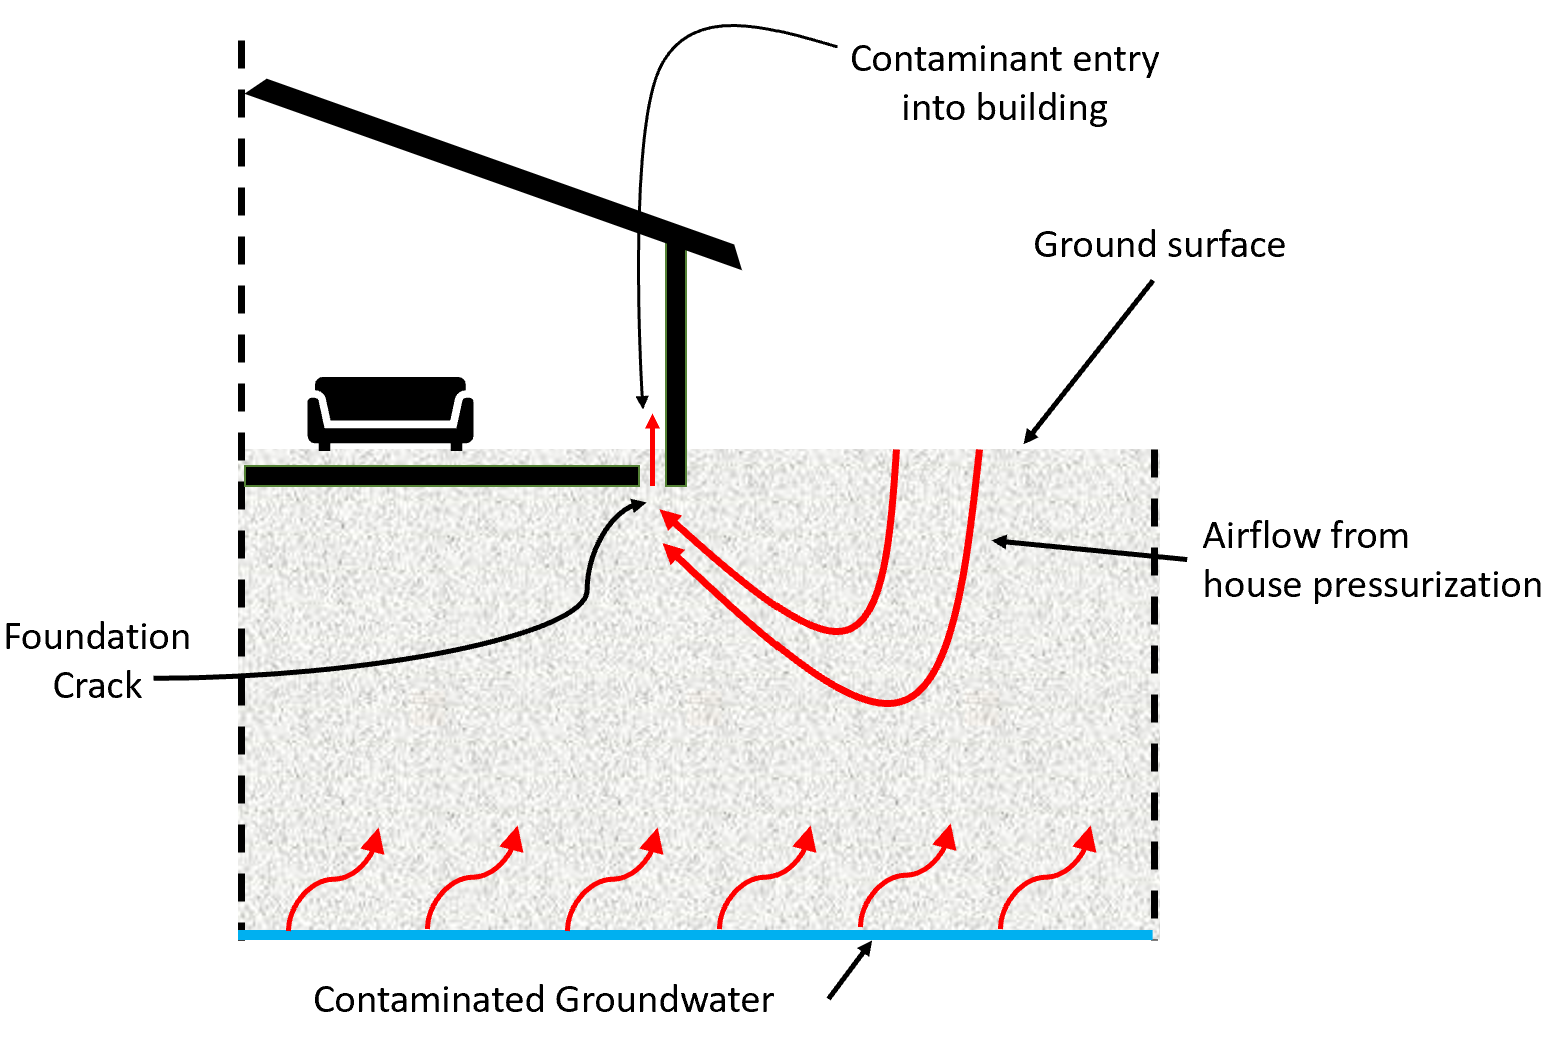
\includegraphics[width=\textwidth]{model_cartoon.png}
  \caption{The considered VI scenario.}
  \label{fig:vi_scenario}
\end{figure}

The basement interior will be modeled as a continuously stirred tank reactor (CSTR), (but without reactions), where the indoor contaminant concentration will depend on the contaminant entry rate $n_\mathrm{ck}$ from the soil via the foundation crack and the air exchange rate $A_e$.
The details of this will be covered section \ref{sec:indoor}.\par

To determine $n_\mathrm{ck}$ the contaminant transport in the soil needs to be modeled.
This will be done using the advection-diffusion equation, which will be modified for transport in soils.
The contaminant transport itself is driven by a concentration gradient and airflow in the soil.
The contaminant source (groundwater) and sink (atmosphere and contaminant entry into the building) will largely determine the concentration gradient, while the airflow needs to be calculated separately.\par

The airflow in the soil is modeled by Darcy's Law, and is driven by a pressure gradient in the soil, which induced by the indoor/outdoor pressure difference.
Details are in section \ref{sec:darcys_law}.\par

One last consideration is that the vadose zone is partially saturated with water, with the soil pores more or less filled near the groundwater interface, and with soil moisture content decreasing as a function of elevation above groundwater $z$ [\si{\metre}].
The soil moisture content has a profound effect on transport in the soil; it restricts both the airflow and contaminant diffusivity in the soil.
Thus, the soil moisture content $\theta_w$ must first be determined in order to solve the contaminant transport and Darcy's Law.\par

The resulting physical system is highly coupled, with many physical aspects dependant on others.
Figure \ref{fig:physics_overview} shows the coupling between each physicsal process, its output, and how it relates to the other processes that ultimately determine VI.\par

% TODO Add Millington-Quirk blob
\begin{figure}
  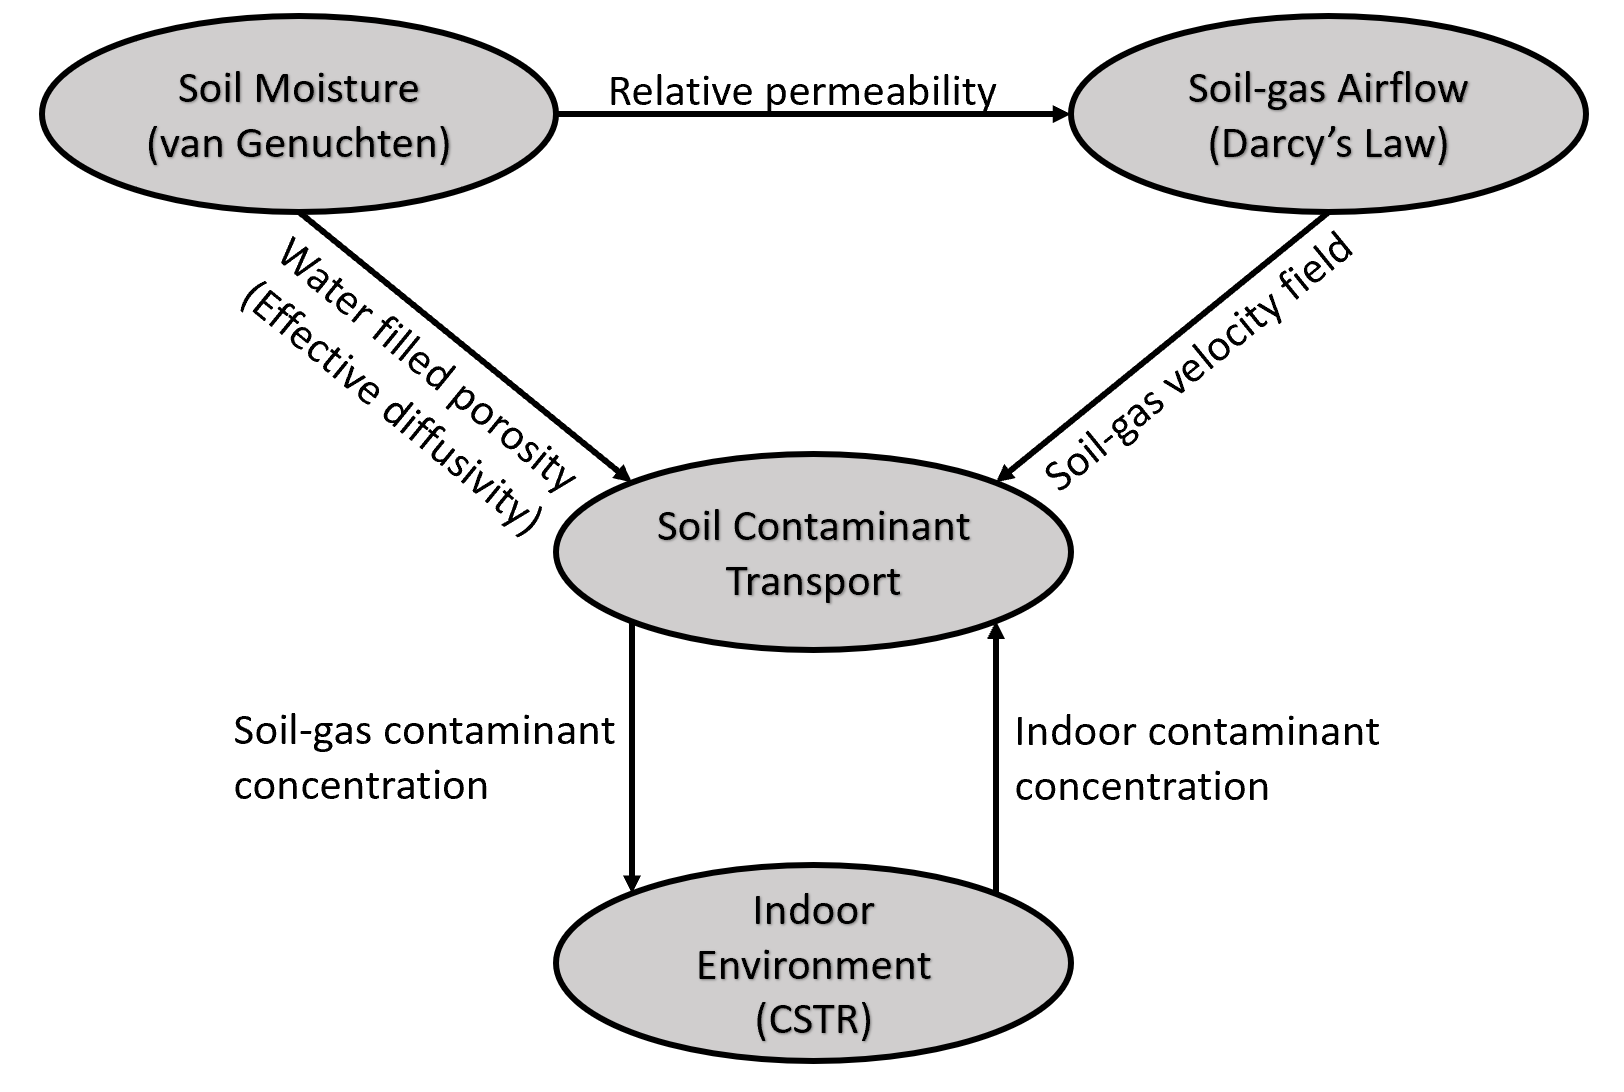
\includegraphics[width=\textwidth]{physics_interaction.png}
  \caption{Coupling between the physics used to model VI.}
  \label{fig:physics_overview}
\end{figure}

In this chapter, we will walk through the process of numerically modeling this VI scenario using the finite element method (FEM) and post-processing of the results.
A discussion regarding past and present VI models, their advantages and limitations, will follow.\par

\subsection{Finite Element Method}

% TODO Make it clear which sources I use here and say so early.
% TODO Make a figure showing the basis functions with nodal coefficients.

Many physical phenomena are described by partial differential equations (PDEs), but for anything but the simplest scenarios, these do not have an analytical closed-form solutions; therefore numerical methods are needed for finding an approximate solution.
This is achieved by discretizing the problem, i.e. transforming a continuous problem into a discrete one.
There are numerous ways to discretize a problem, and some of the more popular schemes are finite difference (FDM), finite volume (FVM), and finite element method (FEM).\par

In this work we use FEM, which is a popular numerical scheme that offers some distinct advantages over other schemes for modeling VI.
FEM subdivides the domain of the PDE problem into many smaller subdomains called elements.
These elements can take a wide variety of shapes, e.g. tetrahedra, prisms, or cuboids for three-dimensional problems and triangles or rectangles for two-dimensional problems.
The collection of elements that make up the domain or geometry is called a \textit{mesh}.
The fineness of the mesh is what largely determines the accuracy of the solution, but also increases the computational costs.\par

The size of each element can be highly nonuniform which allows FEM to discretize complicated geometries.
This is advantageous for modeling VI, where different parts of the geometry can have dramatically different resolution requirements; the \SI{1}{\centi\metre} foundation crack requires elements on the scale of \si{\milli\metre}, while in other parts of the geometry the resolution requirement is on the scale of \si{\metre}.
This ability to easily represent complicated geometries with elements of ununiform sizes helps maintain accuracy while saving computational resources.
Another benefit of using these elements is that it is easy to assign different constant values throughout the domain, and heterogenous materials can easily be represented.\par

The purpose of this work is not to provide a detailed description of the FEM, but for the interested reader \citeauthor{larson_finite_2010}\cite{larson_finite_2010} is a good resource.
However, it is important to know that FEM assumes that the approximated solution to a PDE can be written as a series of linear functions, called \textit{basis functions}.
\begin{equation}
  u \approx u_h = \sum^i u_i \psi_i
\end{equation}
here $u$ is the exact solution to the problem;
$u_h$ is the approximate solution;
$u_i$ is a \textit{nodal coefficient};
and $\psi$ is a \textit{basis function}.
These basis functions are usually some simple function, e.g. a hat function or some lower-order polynomial.\par

These basis functions are used to discretize the problem by rewriting a PDE into its \textit{weak form}, multiplying the equation with another set of functions called a \textit{test function}.
The test functions are the same type of function as the basis function, i.e. if the basis function is a hat function, so is the test function.
The result of this is an integral, where the integrands are the product of the basis function.
These integrals are numerically solved using some quadrature method, which gives a linear system of equations.
This system of equations is then solved to give all of the $u_i$ coefficients and thus the approximated solution $u_h$.\par

The point of this is that choice of basis function, i.e. hat function, first or third order polynomial, can influence the accuracy of the solution, and certain basis functions are more appropriate for certain PDEs.
Generally, higher order polynomials will give a more accurate solution, but at a computational cost, making it sometimes difficult to choose.
This adds another level of complexity of using FEM over some other numerical schemes, as the accuracy of the solution is not only influenced by the mesh but also somewhat by the choice of basis functions.
This highlights one of the drawbacks of FEM, i.e. that it is mathematically more challenging to implement and use than some other numerical schemes may be.\par

Fortunately, due to the attractiveness of the method, many commercial FEM packages have developed which increases usability significantly.
In this work we will use such a package - COMSOL Multiphysics, where subsequent sections will cover the steps required to implement our VI model in COMSOL.
(Of course, this could easily be translated into use in another software package.)\par

In order, we will cover:
\begin{enumerate}
  \item Creation of a model geometry.
  \item Defining physics/governing equations, boundary, and initial conditions.
  \item Discretize/mesh the geometry.
  \item Solver configuration.
  \item Post-process the results.
\end{enumerate}

\section{Geometry Generation}

Designing a good model geometry is critical as it can save significant computational resources.
When designing a geometry the FEM user should try to represent the model geometry as accurately as possible while:
\begin{enumerate}
  \item Avoid unnecessarily fine details; these may require an excessively fine mesh to resolve.
  \item Leverage symmetry to reduce the domain size over which solution must be effected, and thereby the mesh can be made finer in a smaller portion of the domain.
\end{enumerate}\par
Achieving these goals is not always straightforward, and success depends on the skill of the modeler and on the available tools.
Typically a model geometry is constructed in some computer assisted design (CAD) software, and the particular tools available in these packages vary.
While not absolutely necessary, the usa of a CAD package outside of the COMSOL solver might sometimes make development of the domain description easier.\par

\begin{figure}[htb!]
  \centering
  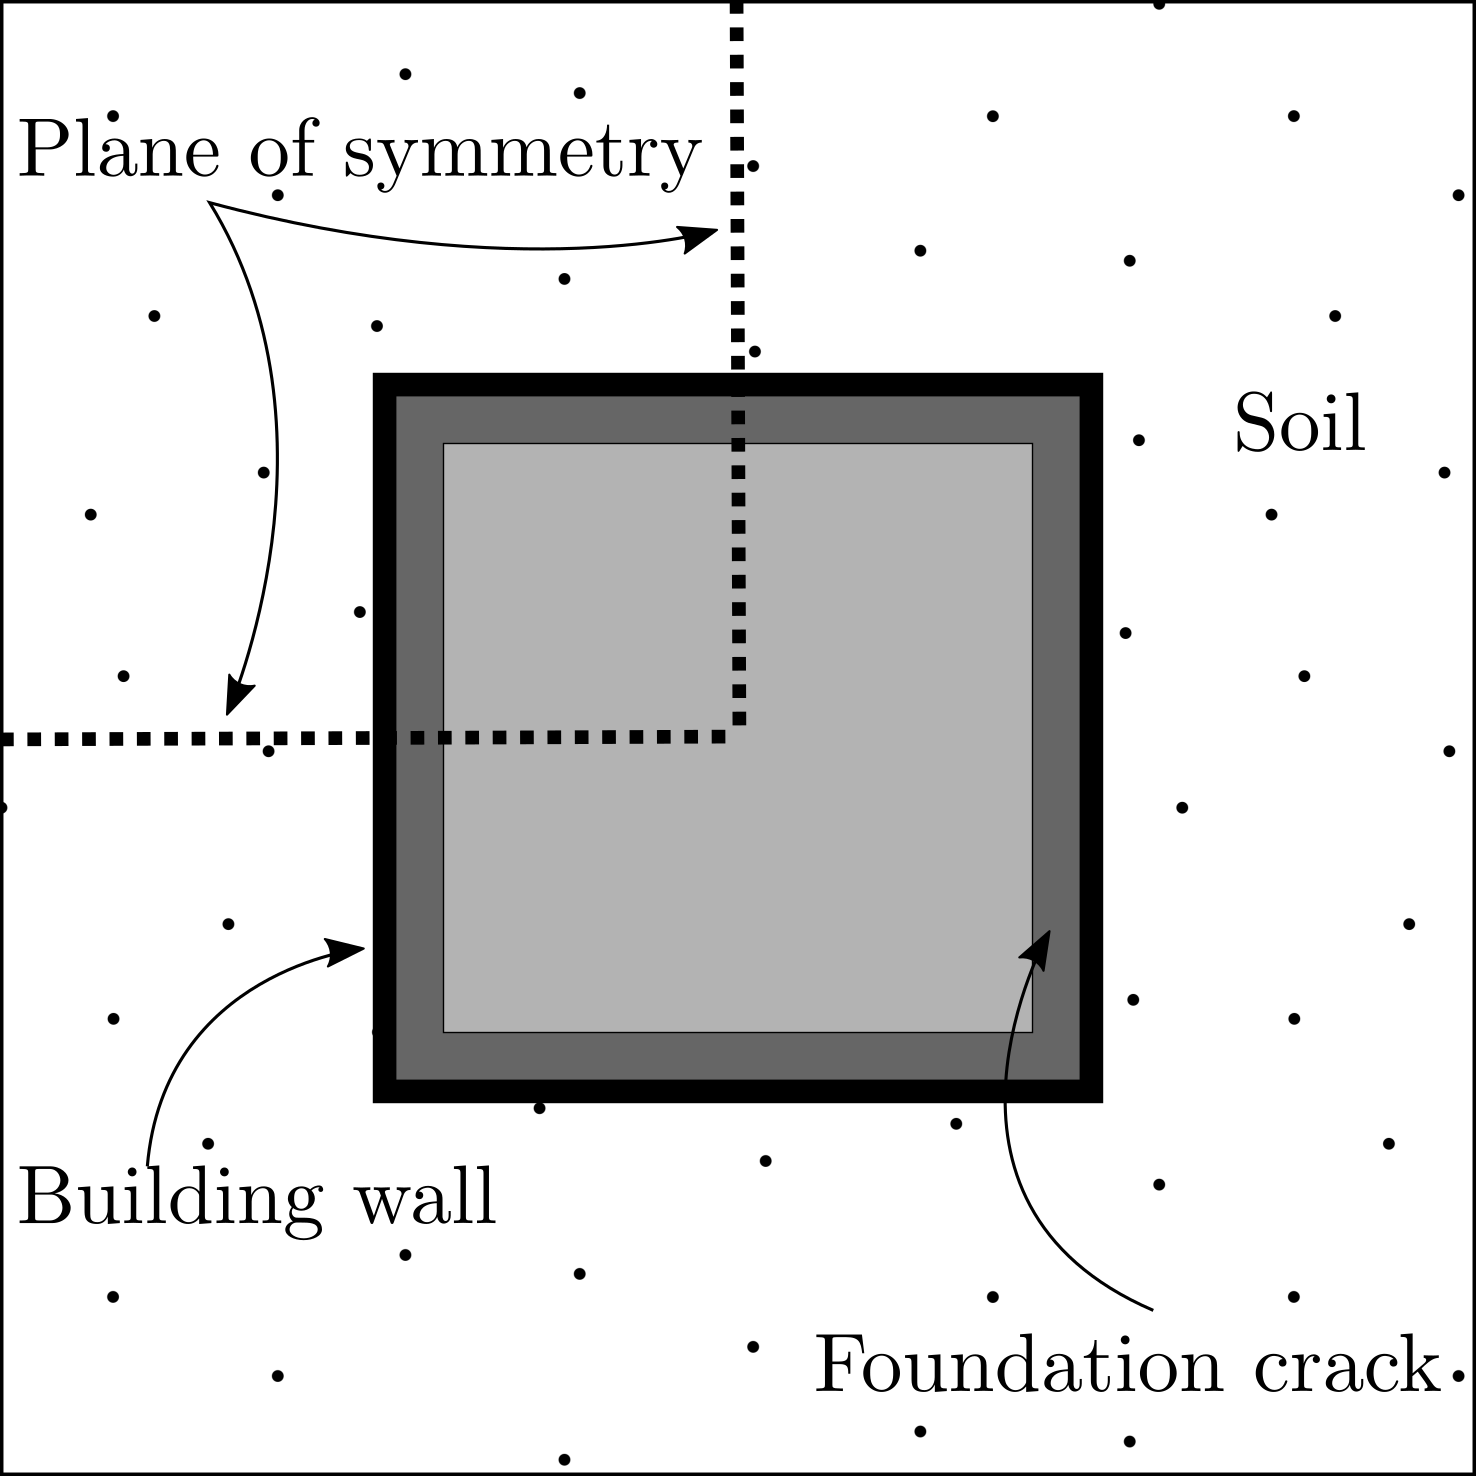
\includegraphics[width=0.75\textwidth]{symmetry.png}
  \caption{Birds-eye view of the VI scenario, showing the foundation and the breach, building wall, as well as the plane of symmetry that allows only a quarter of the total domain to be generated.}
  \label{fig:symmetry}
\end{figure}

COMSOL has a built-in geometry generation tool, which allows the construction of advanced geometries by performing various operations on simpler geometries, e.g. a cylinder and half sphere can be combined to make a rivet.
But as noted, it is also possible to import pre-generated geometries from other CAD software.
For present illustrative purposes, we will create our own geometry.\par

The interior of the house itself will not be explicitly modeled, instead we only consider the soil surrounding the house.
This is done for the simple reason that it is not important to model the interior of the house.
Once the contaminant is in the structure, the damage, so to speak, has been done.
We are interested in how fast the contaminant enters from the soil, which is what determines indoor contaminant concentration.
In addition, typical building interiors are simply too heterogenous to generalize in any meaningful way.
Trying to explicitly model the interior so as to offer insights into indoor concentration variations while at the same time modeling the necessary subsurface transport, would be prohibitively expensive.
Instead the interior is implicitly modeled as a CSTR and simply coupled with the explicit soil and foundation geometry via the foundation crack boundary.\par

One of the nice properties of the described VI scenario is that, due to symmetry, we only need to explicitly model a quarter of it (see Figure \ref{fig:symmetry}).
This reduces the number of required mesh points by 75\%, which is a huge computational saving.
To create the specified geometry, see the instructions for geometry generation in the appendix.

\begin{figure}[htb!]
  \centering
  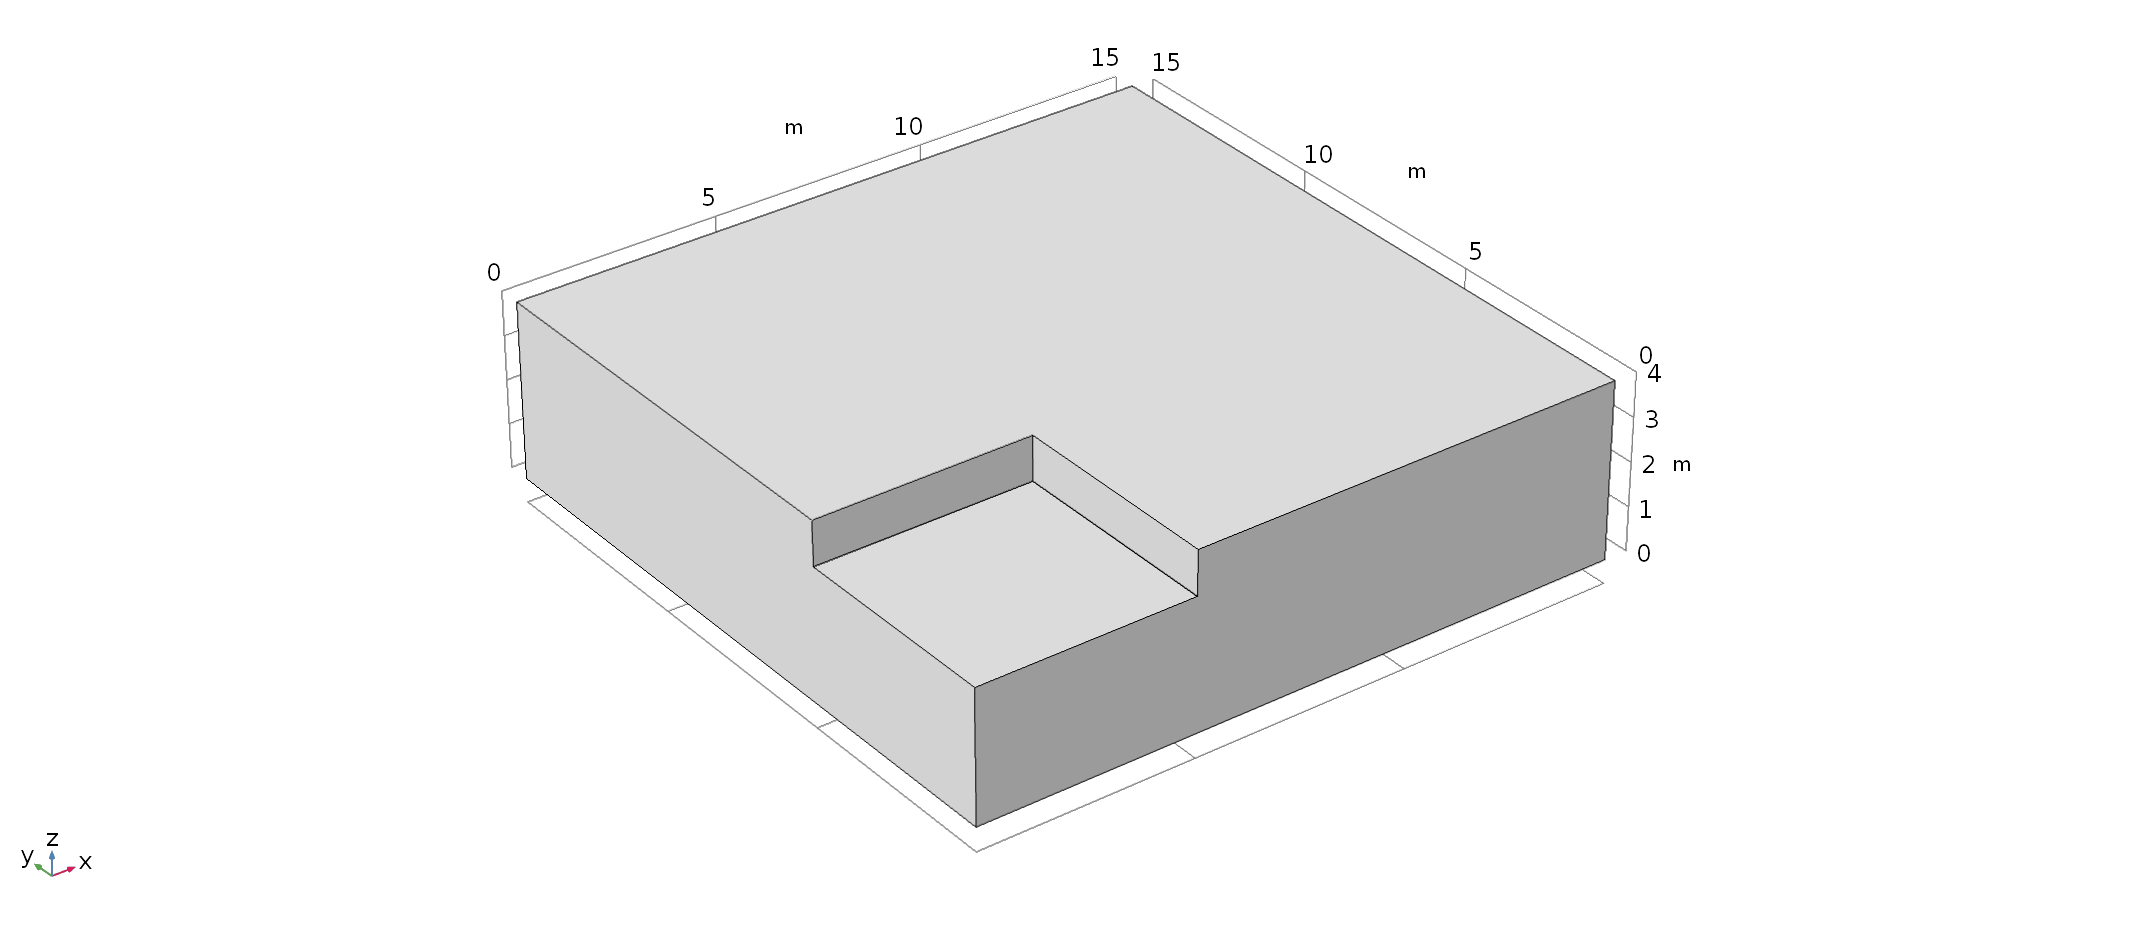
\includegraphics[width=\textwidth]{vi_model.png}
  \caption[VI model geometry in COMSOL]{The complete geometry of the VI scenario as implemented in COMSOL.}
  \label{fig:geometry}
\end{figure}

\subsection{The Indoor Environment}\label{sec:indoor}

The impacts on the indoor air space is perhaps the most important part of modeling VI, as the goal of these models ultimately is to predict indoor exposure given some external factors.
The indoor environment is, however, only modeled implicitly as a continuously stirred tank reactor (CSTR).
We assume that all contaminant entry into the house occurs via a foundation crack.
It has been shown in other modeling work that results are not overly sensitive to the nature and position of the actual foundation breach\cite{yao_simulating_2013}, so we do not need to be overly concerned about the nature of the crack - the key feature is the overall area that it presents for contaminant entry.
Once the contaminant enters the interior, it is instantly perfectly mixed, which is a key assumption of a CSTR.
Contaminant expulsion occurs via air exchange with the outdoor environment, and is regulated by \textit{air exchange rate} $A_e$, which dictates what fraction of the indoor air is exchanged with outdoor air over a given period of time.
For instance, a common air exchange rate for a house is $A_e = \SI{0.5}{\per\hour}$, i.e. half of the indoor air is exchanged every hour.
The impacts of air exchange rate will be explored in Chapter \ref{chp:preferential_pathways}.\par

It should be noted that in this simple VI model implementation, we assume that there are no indoor sources nor that any sorption of contaminant to/from any indoor materials occurs.
Thus, the reaction term that would ordinarily be part of a CSTR is dropped (but is reintroduced in Chapter \ref{chp:sorption}) and the temporal change in indoor contaminant concentration is thus given by \eqref{eq:cstr}.
\begin{equation}\label{eq:cstr}
  V_\mathrm{bldg}\frac{\partial c_\mathrm{in}}{\partial t} = n_\mathrm{ck} - V_\mathrm{bldg} A_e c_\mathrm{in}
\end{equation}
Here $c_\mathrm{in}$ [\si{\mol\per\metre\cubed}] is the indoor air contaminant concentration;
$n_\mathrm{ck}$ [\si{\mol\per\second}] is the contaminant entry (or exit) rate into the building via the foundation crack;
$A_e = \SI{0.5}{\per\hour}$ is the air exchange rate;
Finally, $V_\mathrm{bldg} = \SI{300}{\metre\cubed}$ is the volume of the house interior (or basement in this case).\par

A limitation of this approach is that we only consider one control volume or compartment, while in reality indoor contaminant concentrations can vary significantly between compartments, in particular between different floors.
There are VI models that use multiple compartments, which in essence are just coupled CSTRs\cite{murphy_multi-compartment_2011}.
Basements typically have higher indoor contaminant concentrations than other floors, so in this implementation we assume that our sole compartment is the house basement, which $V_\mathrm{bldg} = \SI{300}{\metre\cubed}$ reflects.\par

Solving \eqref{eq:cstr} requires us to determine the contaminant entry and air exchange rates.
Air exchange rates can vary quite significantly, and are a significant source of temporal variability in VI, a topic that will be further explored in Chapter \ref{chp:preferential_pathways}.
However, they typically vary around relatively well-known values as air exchange rates are regulated in building codes.
For residential buildings, it is typical that air exchange rate is around $A_e = \SI{0.5}{\per\hour}$ and thus for simplicity we will choose this value.\par

\paragraph{Contaminant entry into the building}

Contaminant entry rates are significantly more difficult to determine, as they depend on air velocity through the foundation breach and the concentration gradient across it.
The determination of these is the main point, and challenge in VI modeling.\par

\begin{figure}[htb!]
  \centering
  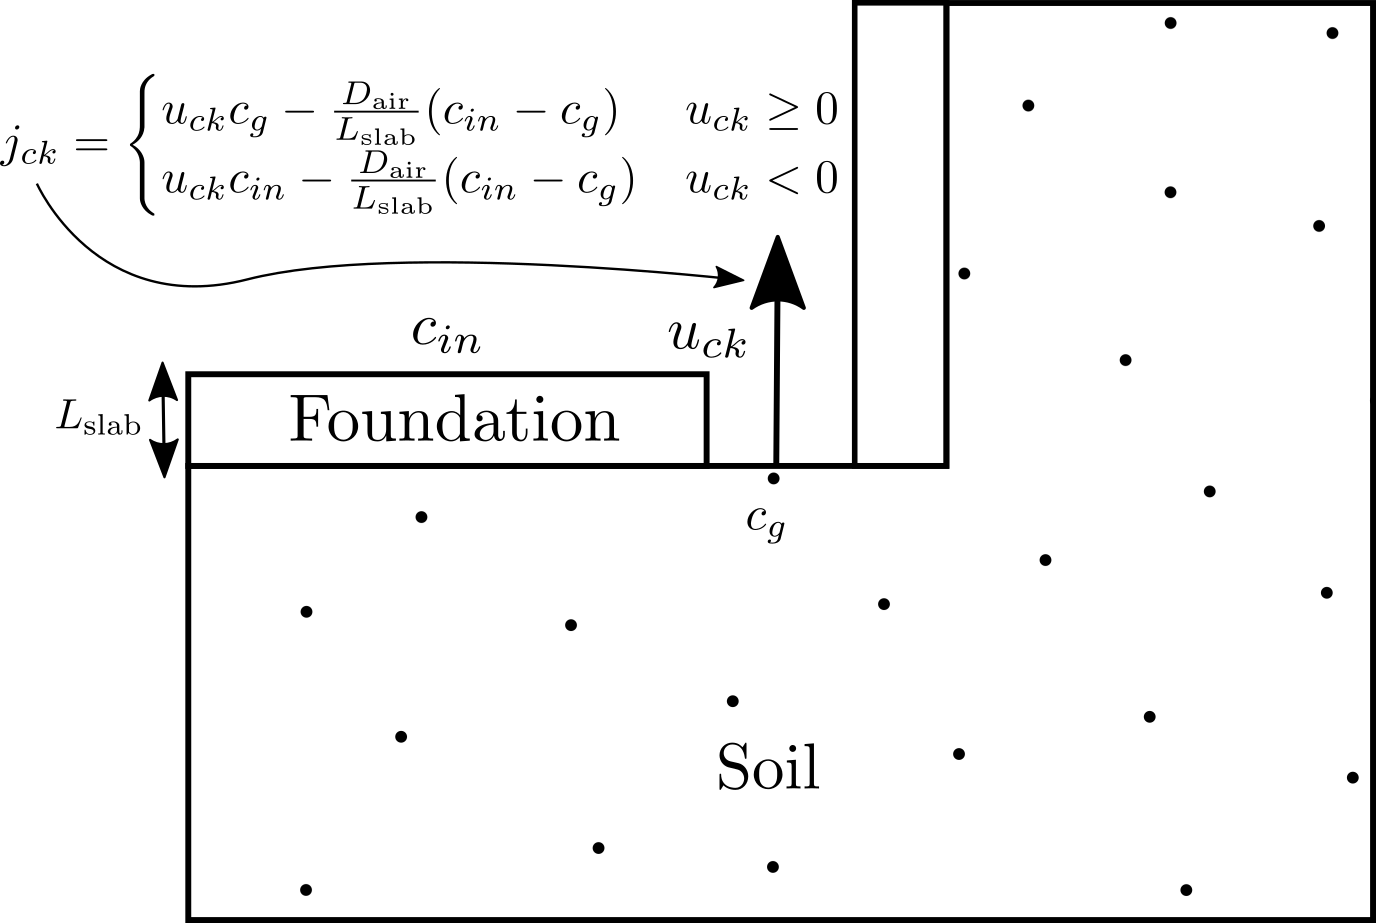
\includegraphics[width=0.6\textwidth]{crack_transport.png}
  \caption[Schematic of soil-gas contaminant entry into a building through a breach in the foundation.]{Soil-gas contaminant vapors are transported from the underlying soil into a building via a breach in the foundation. The scale is exaggerated, and in our modeled scenario the crack is only \SI{1}{\centi\metre} wide.}
  \label{fig:crack_transport}
\end{figure}

The contaminant entry $n_\mathrm{ck}$ is given by integrating the contaminant entry flux $j_\mathrm{ck}$ across the foundation crack boundary $A_\mathrm{ck}$.
\begin{equation}
  n_\mathrm{ck} = \int_{A_\mathrm{ck}} j_\mathrm{ck} dA
\end{equation}
The contaminant flux through the foundation crack is modeled as transport between two parallel plates and has an advective and a diffusive component.
\begin{equation}
  j_\mathrm{ck} = j_\mathrm{advection} + j_\mathrm{diffusion}
\end{equation}
Since contaminant concentration indoors is lower than it is in the soil or near foundation crack region a concentration gradient from the soil-gas to the indoor will exist.
The interior of the crack is not explicitly modeled, but assumed to only contain air and thus we assume the diffusion coefficient is the same as in air.
\begin{equation}
  j_\mathrm{diffusion} = - \frac{D_\mathrm{air}}{L_\mathrm{slab}} (c_{in} - c_g)
\end{equation}
here $D_\mathrm{air} = \SI{7.2e-6}{\metre\squared\per\second}$ is the diffusion coefficient of TCE in air as a sample contaminant of interest; other contaminant of common concern have comparable diffusivities.
$L_\mathrm{slab} = \SI{15}{\centi\metre}$ is a typical thickness of a foundation slab;
$c_{in}$ [\si{\mol\per\metre\cubed}] is the indoor contaminant concentration;
$c_g$ [\si{\mol\per\metre\cubed}] is the contaminant gas-phase concentration at the foundation crack boundary.\par

Advective transport through the slab can occur in both directions, i.e. contaminants can be carried from the soil into the house and from the house into the soil\cite{holton_creation_2018}.
The direction of this transport depend on the direction of the flow, with a positive sign indicating that airflow goes into the house.
\begin{equation}
  j_{advection} = \begin{cases}
    u_{ck} c_g & u_{ck} \geq 0 \\
    u_{ck} c_{in} & u_{ck} < 0
\end{cases}
\end{equation}
here $u_{ck}$ [\si{\metre\per\second}] is the airflow velocity through the foundation crack.

Thus the total contaminant transport through the foundation crack is given by \eqref{eq:contaminant_entry}.
\begin{equation}\label{eq:contaminant_entry}
  j_{ck} = \begin{cases}
    u_{ck} c_g - \frac{D_\mathrm{air}}{L_\mathrm{slab}} (c_{in} - c_g) & u_{ck} \geq 0 \\
    u_{ck} c_{in} - \frac{D_\mathrm{air}}{L_\mathrm{slab}} (c_{in} - c_g) & u_{ck} < 0
\end{cases}
\end{equation}
(See Figure \ref{fig:crack_transport}.)
Not only will \eqref{eq:contaminant_entry} be used to calculate the contaminant entry rate into house, but it is a necessary boundary condition for calculating the contaminant concentration in the soil.
However, as we see, \eqref{eq:contaminant_entry} is a function of both the soil-gas concentration at the foundation crack boundary $c_g$ and the indoor contaminant concentration $c{in}$, thus these two are coupled and need to be solved simultaneously.\par


\section{Water Flow in Unsaturated Porous Media}
\subsection{Water Flow in Unsaturated Porous Media}\label{sec:richards}


\subsubsection{Soil-Water Potential}

\subsubsection{Soil-Water Retention Curve}

The distribution of soil moisture in the soil matrix has profound implications for the advective and diffusive transport of contaminants.
Soil has a limited amount of pore volume available for contaminant transport, and the presence of water restricts this further; decreasing permeability of the soil and subsequently reduces air flow.
Diffusivity of the contaminant will also be retarded by the water.
The contaminant will dissolve into and evaporate from water and the transport will partially occur through water.
Liquid diffusion coefficients are usually around four orders of magnitude smaller than in air.

The soil moisture content of soils can be estimated in many ways, but two common approaches is to use the analytical formulas of \textit{van Genuchten} or \textit{Brooks and Corey}.
Both of these formulas give the soil moisture content as a function of the fluid pressure head, $H_p$.
By definition, when the pressure head is equal to or greater than zero, $H_p \geq 0$, the soil is assumed to be 100\% saturated with the fluid.
In this work, \textit{van Genuchten's} formula is used.

The soil moisture content, $\theta$ is given by.
\begin{equation}
  \theta = \begin{cases}
    \theta_r + \mathrm{Se}(\theta_s - \theta_r) & H_p < 0 \\
    \theta_s & H_p \geq 0
\end{cases}
\end{equation}

The saturation is given by.
\begin{equation}
  \mathrm{Se} = \begin{cases}
    \frac{1}{(1 + |\alpha H_p|^m)^m} & H_P < 0 \\
    1 & H_p \geq 0
  \end{cases}
\end{equation}

\begin{equation}
  C_m = \begin{cases}
    \frac{\alpha m}{1-m}(\theta_s - \theta_r)\mathrm{Se}^{\frac{1}{m}}\big( 1 - \mathrm{Se}^{\frac{1}{m}} \big)^m & H_p < 0 \\
    0 & H_p \geq 0
  \end{cases}
\end{equation}

\begin{equation}
  k_r = \begin{cases}
    \mathrm{Se}^l \big[ 1 - \big( 1 - \mathrm{Se}^\frac{1}{m} \big) \big]^2 & H_p < 0 \\
    0 & H_p \geq 0
  \end{cases}
\end{equation}


% Theory soil-water potential and its modeling with Richard's equation
\subsection{Soil-Water Potential}

% van Genuchten's equation
\subsection{Soil-Water Retention Curve}
\subsubsection{Soil-Water Retention Curve}

The distribution of soil moisture in the soil matrix has profound implications for the advective and diffusive transport of contaminants.
Soil has a limited amount of pore volume available for contaminant transport, and the presence of water restricts this further; decreasing permeability of the soil and subsequently reduces air flow.
Diffusivity of the contaminant will also be retarded by the water.
The contaminant will dissolve into and evaporate from water and the transport will partially occur through water.
Liquid diffusion coefficients are usually around four orders of magnitude smaller than in air.

The soil moisture content of soils can be estimated in many ways, but two common approaches is to use the analytical formulas of \textit{van Genuchten} or \textit{Brooks and Corey}.
Both of these formulas give the soil moisture content as a function of the fluid pressure head, $H_p$.
By definition, when the pressure head is equal to or greater than zero, $H_p \geq 0$, the soil is assumed to be 100\% saturated with the fluid.
In this work, \textit{van Genuchten's} formula is used.

The soil moisture content, $\theta$ is given by.
\begin{equation}
  \theta = \begin{cases}
    \theta_r + \mathrm{Se}(\theta_s - \theta_r) & H_p < 0 \\
    \theta_s & H_p \geq 0
\end{cases}
\end{equation}

The saturation is given by.
\begin{equation}
  \mathrm{Se} = \begin{cases}
    \frac{1}{(1 + |\alpha H_p|^m)^m} & H_P < 0 \\
    1 & H_p \geq 0
  \end{cases}
\end{equation}

\begin{equation}
  C_m = \begin{cases}
    \frac{\alpha m}{1-m}(\theta_s - \theta_r)\mathrm{Se}^{\frac{1}{m}}\big( 1 - \mathrm{Se}^{\frac{1}{m}} \big)^m & H_p < 0 \\
    0 & H_p \geq 0
  \end{cases}
\end{equation}

\begin{equation}
  k_r = \begin{cases}
    \mathrm{Se}^l \big[ 1 - \big( 1 - \mathrm{Se}^\frac{1}{m} \big) \big]^2 & H_p < 0 \\
    0 & H_p \geq 0
  \end{cases}
\end{equation}


% Darcy's Law
\section{Vapor Transport in Unsaturated Porous Media}
\subsection{Vapor Transport in Unsaturated Porous Media}\label{sec:darcys}

Fluid transport in porous media is governed by \textit{Darcy's Law} and was originally formulated by Henry Darcy based on his work on describing water flow through soil under the influence of gravity.
Since then it been found to derivable in several ways from the Navier-Stokes equations\cite{bear_dynamics_1972} and may be stated as a pressure gradient driven velocity.
\begin{equation}\label{eq:darcys_law_saturated}
  \vec{u} = -\frac{\kappa}{\mu}\nabla p
\end{equation}
Here $\vec{u}$ is the fluid velocity; $\kappa$ the soil permeability; $\mu$ is the fluid viscosity; and $\nabla p$ is the pressure gradient.
In VI modeling we're interested in the flow of contaminant vapors but since the contaminant concentrations are typically very low, the transport properties may be taken from those of pure air.\par

% TODO: Elaborate on the assumptions, i.e. that in DL the viscosity shear effects may be neglected. But this breaks down when Re is too high.

For Darcy's Law to be valid, two assumptions must be fulfilled:
\begin{enumerate}
  \item The fluid must be in the laminar regime, typically $\mathrm{Re} < 1$.
  \item The soil matrix must be saturated with the fluid.
\end{enumerate}
Typically the vapor flows in most VI scenarios are sufficiently slow for the first condition to be fulfilled.
And if they are not, there are modifications to Darcy's Law that
Most of the contaminant vapor transport takes place in the partially saturated vadose zone and thus, \eqref{eq:darcys_law_saturated} needs modification.\par

In partially saturated soils, a varying portion of the soil pores are available for vapor transport, with the rest being occupied by water, affecting the effective permeability of the soil.
To model this, we use the relative permeability property, $k_r$, from section \ref{sec:richards} is used.
\begin{equation}
  \kappa_\mathrm{eff} = (1-k_r) \kappa_s
\end{equation}
Note that in this Darcy's formulation $(1 - k_r)$ is used to refer to the relative permeability of vapor, e.g. that 0 indicates the soil is completely impermeable for vapor flow (and vice versa).\par
This gives the modified Darcy's Law used in VI-modeling:
\begin{equation}\label{eq:darcys_law}
  \vec{u} = -\frac{(1-k_r) \kappa_s}{\mu}\nabla p
\end{equation}

However, \eqref{eq:darcys_law} only gives the vapor velocity as a function of the pressure gradient, to properly model the vapor flow in the soil matrix we need to incorporate Darcy's Law into a continuity equation giving
\begin{equation}\label{eq:vapor_transport}
  \frac{\partial}{\partial t} (\rho \epsilon) + \nabla \cdot \rho \Big( -\frac{(1-k_r) \kappa_s}{\mu} \nabla p \Big) = Q_m
\end{equation}
which is governing equation for vapor flow in porous media.\par

\paragraph{Boundary conditions}

In order to solve \eqref{eq:vapor_transport} we need to define some boundary conditions.
In our CSM, air is pulled from the atmosphere through the ground surface and into the building via the foundation crack.
To model this only three boundary conditions are required.\par

The first is to define a pressure gauge, i.e. a reference point for where the pressure is zero, which is where air will be pulled from.
This is the applied to the ground surface boundary.
The second is that we apply the indoor/outdoor pressure difference (~5 Pa) to the foundation crack boundary.
The third type is applied to all remaining boundaries and is a no flow boundary condition, indicating that no flow passes through these boundaries.
We also make sure that we specify the symmetry planes present.
\begin{align}
  &\text{Ground surface} &p = 0 \; \mathrm{(Pa)} \\
  &\text{Foundation crack} &p = p_\mathrm{in/out} = -5 \; \mathrm{(Pa)} \\
  &\text{Remaining} &-\vec{n}\cdot\rho\vec{u} = 0
\end{align}
where $\vec{n}$ is the boundary normal vector.\par


% Mass Transport
\documentclass{article}

\usepackage{amsmath}
\usepackage[utf8]{inputenc}


\begin{document}

\section{Mass Transport in Partially Saturated Porous Media}

The vadose zone is a three-phase system and thus any chemical specie is distributed between these three phases.
However, the mass transport still only occur through the gas and liquid phases of the system, therefore the transport of the \textit{total} concentration $c_T$ is due to diffusive and advective transport in these phases.
\begin{equation}\label{eq:mass1}
  \frac{\partial c_T}{\partial t} = \nabla [D_w \theta_w \tau_w \nabla c_w + D_g \theta_g \tau_g \nabla c_g]
    - \nabla (v_w \theta_w c_w + v_g \theta_g c_g)
\end{equation}
Here $D_w$ and $D_g$ are the water and gas diffusion constants respectively; $\theta_w$ and $\theta_g$ are the water and gas filled porosities; $\tau_w$ and $\tau_g$ are the tortuosity, correcting for diffusivity in porous media; $v_w$ and $v_g$ are the water and gas velocity; finally $c_w$ and $c_g$ are the water and gas phase concentrations.\par

As stated above, the total concentration is distributed across the three phases.
\begin{equation}
  c_T = \theta_w c_w + c_g \theta_g + c_s \rho_b
\end{equation}
Where the first and second terms correspond to the water and gas concentrations; the third correspond to the sorbed concentration, where $c_s$ is the sorbed concentration by mass and $\rho_b$ is the soil bulk density.
In order to solve \eqref{eq:mass1} we need to state everything in terms of one dependent variable, which we will see is the water concentration $c_w$.

From Henry's Law we know that a gas concentration is proportional to the water concentration via the eponymous constant $H$.
\begin{equation}
  c_g = H c_w
\end{equation}
By assuming linear sorption we can describe the sorbed concentration as
\begin{equation}
  c_s = \begin{cases}
    K_p c_w &\text{Water phase sorption} \\
    K_p c_g = K_p H c_w &\text{Gas phase sorption}
  \end{cases}
\end{equation}
where $K_p$ is the sorption isotherm.
For simplicity we will here assume water phase sorption.

Using this we can restate $c_T$ is terms of the water phase concentration.
\begin{equation}
  c_T = (\theta_w + \theta_g H + K_p \rho_b) c_w = R c_w
\end{equation}
The \textit{retardation factor} $R$ is introduced to simplify writing.

Now we substitute all of this in \eqref{eq:mass1}.
\begin{equation}\label{eq:mass2}
  R \frac{\partial c_w}{\partial t} = \nabla [(D_w \theta_w \tau_w + D_g \theta_g \tau_g H)\nabla c_w]
    - \nabla [(v_w \theta_w + v_g \theta_g H) c_w]
\end{equation}
Here we recognize that $(D_w \theta_w \tau_w + D_g \theta_g \tau_g H)$ is the effective diffusivity $D_\mathrm{eff}$, which gives the final expression
\begin{equation}\label{eq:mass3}
  R \frac{\partial c_w}{\partial t} = \nabla [D_\mathrm{eff} \nabla c_w]
    - \nabla [(v_w \theta_w + v_g \theta_g H) c_w]
\end{equation}

Most soil-physics books are concerned with water moving in porous media, with the gas assumed to be immobile and occupy small pockets in the porous media.
In this case $v_g = 0$, dropping that term which gives
\begin{equation}\label{eq:mass4}
  R \frac{\partial c_w}{\partial t} = \nabla [D_\mathrm{eff} \nabla c_w]
    - \nabla [v_w \theta_w c_w]
\end{equation}
This is the most common form found of the governing equation for mass transport in partially saturated porous media, and the equation that COMSOL solves.

Obviously this does not quite describe the vapor intrusion scenario, where we are concerned with a mobile gas phase and a stationary water phase.
Although, this does not necessarily have to be the case, and we could in theory keep both velocity fields if we were interested in such an problem.
Regardless, for most of our applications we assume that the soil water is stationary $v_w = 0$ leading to
\begin{equation}\label{eq:mass5}
  R \frac{\partial c_w}{\partial t} = \nabla [D_\mathrm{eff} \nabla c_w]
    - \nabla [v_g \theta_g H c_w]
\end{equation}
The implications of this is that we must multiply the gas velocity field with the Henry's Law constant to correctly reflect the transport problem.

Another implication is that \textbf{we must set all our boundary conditions in terms of the water phase concentration} $c_w$.
So for one, the concentration boundary condition at the groundwater source must be the groundwater \textit{water} concentration, and not the typical one where we multiply it by $H$; as we've seen, this previous correction is built into the governing equation.

The crack entry flux $j_{ck}$ must also be adjusted.
This one is a bit trickier though, since we're only concerned the gas phase concentration entering through the crack.
Thus it must be stated as a function of the gas phase concentration, i.e. $j_{ck} = f(c_g)$ and this is the contaminant flux that enters the overlying building.
But since we must state every boundary condition in terms of $c_w$, we must scale the boundary condition in the model using Henry's Law as well, and thus it should be $j_{ck}/H$.

\end{document}



% TODO: Add multiphase theory for NAPL and DNAPL transport in vadose zone?

\section{Meshing}

\section{Solver Configuration}


\section{References}

\end{document}
